\documentclass[10pt,twocolumn,letterpaper]{article}

\usepackage{cvpr}
\usepackage{times}
\usepackage{epsfig}
\usepackage{graphicx}
\usepackage{amsmath}
\usepackage{amssymb}
\usepackage{booktabs}
\usepackage{tikz}
\usepackage{pgfplots}
\pgfplotsset{compat=1.18}
\usetikzlibrary{positioning,arrows.meta,shapes.geometric,fit,calc,decorations.pathreplacing}
\usepackage{multirow}
\usepackage{xcolor}
\usepackage{hyperref}

\definecolor{tcblue}{RGB}{52,152,219}
\definecolor{tcgreen}{RGB}{46,204,113}
\definecolor{tcorange}{RGB}{230,126,34}
\definecolor{tcred}{RGB}{231,76,60}
\definecolor{tcpurple}{RGB}{155,89,182}

\cvprfinalcopy

\def\cvprPaperID{****}
\def\httilde{\mbox{\tt\raisebox{-.5ex}{\symbol{126}}}}

\begin{document}

\title{Temporally Consistent Talking Head Synthesis with Neural Radiance Fields}

\author{
Anonymous CVPR Workshop Submission
}

\maketitle

% ============================================================================
\begin{abstract}
NeRF-based talking head synthesis methods produce high-quality per-frame renderings but suffer from temporal inconsistencies that manifest as flickering artifacts in the generated videos.
This limitation arises because each frame is rendered independently, without explicit supervision for temporal coherence.
We propose three complementary improvements to SyncTalk that address temporal stability: (1) a temporal consistency loss that penalizes frame-to-frame prediction differences, encouraging smooth transitions between consecutive frames; (2) a multi-head self-attention mechanism for audio temporal modeling that replaces the fixed convolutional attention with content-dependent temporal weighting; and (3) a cosine annealing learning rate schedule with warmup for more stable training dynamics.
We additionally introduce an early stopping mechanism to prevent overfitting.
Experiments demonstrate improved temporal stability with reduced flickering while maintaining synthesis quality, as measured by standard metrics (PSNR, LPIPS) and temporal consistency metrics.
\end{abstract}

% ============================================================================
\section{Introduction}

Neural Radiance Field (NeRF)-based talking head methods~\cite{guo2021adnerf, tang2022radnerf, li2023ernerf, peng2024synctalk} have achieved impressive visual quality for single-frame synthesis.
However, when assembled into video, these methods frequently exhibit temporal flickering --- sudden brightness changes, jittering edges, and inconsistent texture details between consecutive frames.

This problem stems from the fundamental per-frame training paradigm: each frame is optimized independently, and the only implicit temporal signal comes from shared network weights.
Small variations in per-frame audio features, sampling noise, and optimization dynamics can produce visible inconsistencies when frames are played sequentially at 25 FPS.

We propose three targeted improvements to SyncTalk~\cite{peng2024synctalk} that enhance temporal consistency:

\begin{enumerate}
    \item \textbf{Temporal Consistency Loss}: A loss that explicitly penalizes frame-to-frame prediction differences in facial regions, encouraging the model to produce smooth transitions.
    \item \textbf{Temporal Audio Attention}: Multi-head self-attention over the audio sequence with positional encoding, enabling content-dependent temporal weighting that adapts to speech dynamics.
    \item \textbf{Cosine LR Schedule with Warmup}: A learning rate schedule that avoids the early instability of the original exponential decay and maintains higher learning rates in the middle of training for better exploration.
\end{enumerate}

% ============================================================================
\section{Related Work}

\paragraph{NeRF-Based Talking Heads.}
Building on Neural Radiance Fields~\cite{mildenhall2020nerf}, methods like AD-NeRF~\cite{guo2021adnerf}, RAD-NeRF~\cite{tang2022radnerf}, ER-NeRF~\cite{li2023ernerf}, and SyncTalk~\cite{peng2024synctalk} condition the radiance field on audio to drive facial animation.
While achieving excellent per-frame quality, none explicitly optimizes for temporal consistency.

\paragraph{Temporal Consistency in Neural Rendering.}
DVS~\cite{regnerf2022} and subsequent works have explored temporal priors for dynamic NeRFs.
In the 2D domain, methods like Blind Video Consistency~\cite{lai2018blind} enforce temporal coherence through optical flow warping.
We adapt the concept of temporal prediction consistency to the talking head setting, where the challenge is balancing stability with natural mouth motion variability.

\paragraph{Attention Mechanisms for Sequential Data.}
Transformer-based attention~\cite{vaswani2017attention} has become standard for modeling temporal dependencies.
For audio-driven animation, the temporal context window determines how much past and future audio influences the current frame.
Our approach replaces the fixed convolutional attention of SyncTalk with content-dependent multi-head self-attention.

% ============================================================================
\section{Methodology}

\subsection{Temporal Consistency Loss}

Given a sequence of frames, we store the previous frame's prediction $\hat{I}_{t-1}$ (detached from the computation graph) and penalize differences with the current prediction $\hat{I}_t$ in the face region:

\begin{equation}
    \mathcal{L}_{\text{temporal}} = \frac{1}{|\mathcal{M}|} \sum_{p \in \mathcal{M}} \|\hat{I}_t(p) - \hat{I}_{t-1}(p)\|_1
\end{equation}

where $\mathcal{M}$ is the face mask. This loss has important design choices:

\begin{itemize}
    \item \textbf{Warmup}: Applied only after $N_{\text{warm}}$ steps to allow the model to learn basic structure first.
    \item \textbf{Face mask}: Applied only to face regions, not background, since the torso is handled by a separate model.
    \item \textbf{Detached target}: The previous prediction is detached to prevent the loss from collapsing to trivial solutions (both predictions going to the same constant).
    \item \textbf{Gradual ramp}: The loss weight increases linearly from 0 to $\lambda_{\text{temp}}$ over training, avoiding early disruption of the learning signal.
\end{itemize}

\subsection{Temporal Audio Attention}

We replace SyncTalk's convolutional attention with a multi-head self-attention mechanism over the audio feature sequence:

\begin{equation}
    \mathbf{h} = \text{LayerNorm}(\mathbf{x} + \text{MultiHead}(\mathbf{x}, \mathbf{x}, \mathbf{x}))
\end{equation}
\begin{equation}
    \mathbf{o} = \text{LayerNorm}(\mathbf{h} + \text{FFN}(\mathbf{h}))
\end{equation}

A learnable query token pools the sequence into a single vector via cross-attention. Sinusoidal positional encoding provides temporal position information.

\subsection{Cosine Learning Rate Schedule}

The original SyncTalk uses exponential decay: $\text{lr}(t) = \text{lr}_0 \cdot 0.5^{t/T}$, which decays monotonically.
We replace this with cosine annealing with linear warmup:

\begin{equation}
    \text{lr}(t) = \begin{cases}
        \text{lr}_0 \cdot \frac{t}{T_w} & t < T_w \\
        \frac{\text{lr}_0}{2}\left(1 + \cos\left(\frac{\pi(t - T_w)}{T - T_w}\right)\right) & t \geq T_w
    \end{cases}
\end{equation}

where $T_w$ is the warmup period. This schedule has three advantages: (1) warmup prevents early training instability when hash grid features are near-random; (2) the cosine curve maintains higher learning rates in mid-training for exploration; (3) smooth decay at the end allows fine convergence.

% Architecture Figure
\begin{figure*}[t]
\centering
\resizebox{0.95\textwidth}{!}{
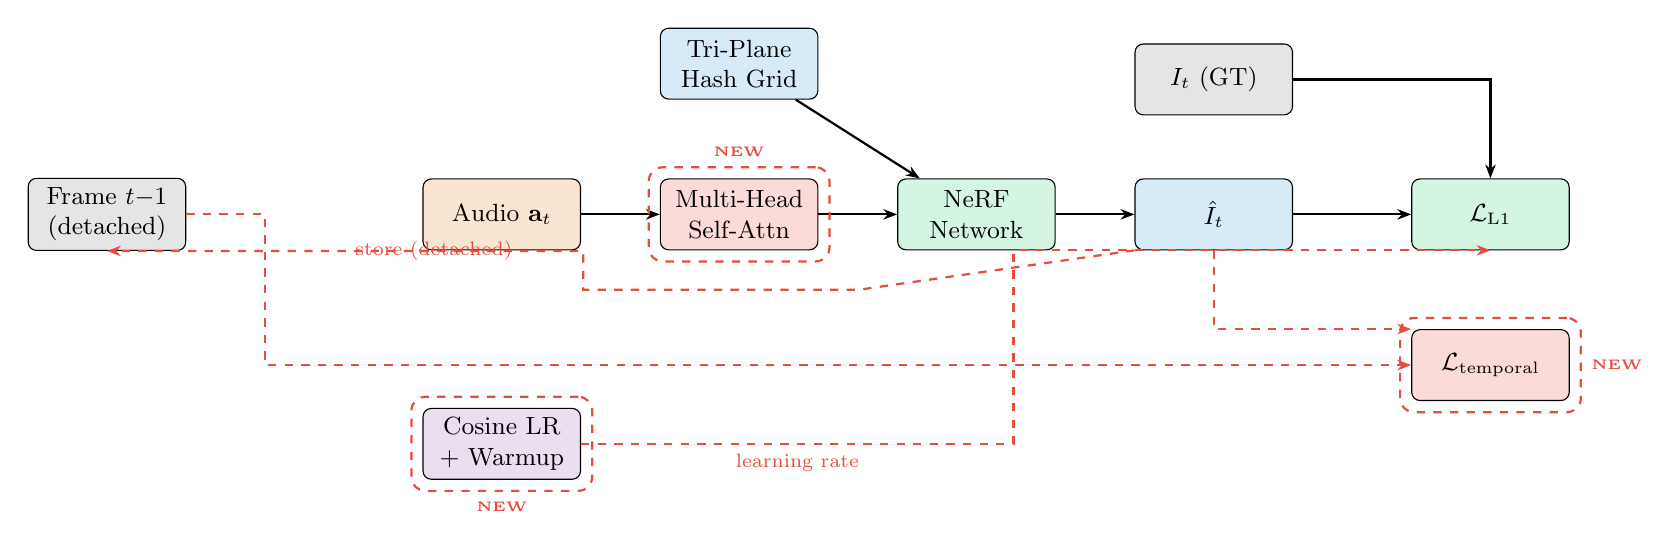
\begin{tikzpicture}[
    block/.style={rectangle, draw, fill=#1!20, minimum height=0.9cm, minimum width=2cm, align=center, rounded corners=3pt, font=\small},
    block/.default=tcblue,
    arrow/.style={-{Stealth[length=5pt]}, thick},
    darrow/.style={-{Stealth[length=5pt]}, thick, dashed, color=tcred},
]

% Frame t-1
\node[block=gray] (prev_frame) {Frame $t{-}1$\\(detached)};

% Frame t pipeline
\node[block=tcorange, right=3cm of prev_frame] (audio_t) {Audio $\mathbf{a}_t$};
\node[block=tcred, right=1cm of audio_t] (self_att) {Multi-Head\\Self-Attn};
\node[block=tcblue, above=1cm of self_att] (triplane) {Tri-Plane\\Hash Grid};
\node[block=tcgreen, right=1cm of self_att] (nerf) {NeRF\\Network};
\node[block=tcblue, right=1cm of nerf] (render_t) {$\hat{I}_t$};

% GT
\node[block=gray, above=0.8cm of render_t] (gt) {$I_t$ (GT)};

% Losses
\node[block=tcgreen, right=1.5cm of render_t] (l1_loss) {$\mathcal{L}_{\text{L1}}$};
\node[block=tcred, below=1cm of l1_loss] (temp_loss) {$\mathcal{L}_{\text{temporal}}$};

% LR Schedule
\node[block=tcpurple, below=2cm of audio_t] (lr_sched) {Cosine LR\\+ Warmup};

% Arrows
\draw[arrow] (audio_t) -- (self_att);
\draw[arrow] (self_att) -- (nerf);
\draw[arrow] (triplane) -- (nerf);
\draw[arrow] (nerf) -- (render_t);
\draw[arrow] (render_t) -- (l1_loss);
\draw[arrow] (gt) -| (l1_loss);

% Temporal loss connections
\draw[darrow] (prev_frame.east) -- ++(1, 0) |- (temp_loss.west);
\draw[darrow] (render_t.south) |- (temp_loss.north west);

% LR influence
\draw[darrow] (lr_sched) -- ++(6.5, 0) node[midway, below, font=\scriptsize, text=tcred] {learning rate} |- (l1_loss.south);

% Store prev frame
\draw[darrow] (render_t.south west) -- ++(-3.5, -0.5) -- ++(-3.5, 0) |- (prev_frame.south) node[near end, right, font=\scriptsize, text=tcred] {store (detached)};

% Highlight new components
\node[draw=tcred, dashed, thick, rounded corners=5pt, fit=(self_att), inner sep=4pt, label={[font=\tiny\bfseries, text=tcred]above:NEW}] {};
\node[draw=tcred, dashed, thick, rounded corners=5pt, fit=(temp_loss), inner sep=4pt, label={[font=\tiny\bfseries, text=tcred]right:NEW}] {};
\node[draw=tcred, dashed, thick, rounded corners=5pt, fit=(lr_sched), inner sep=4pt, label={[font=\tiny\bfseries, text=tcred]below:NEW}] {};

\end{tikzpicture}
}
\caption{\textbf{Temporal consistency framework.} Our three improvements (red dashed): (1) Temporal consistency loss comparing consecutive frame predictions, (2) multi-head self-attention for audio temporal modeling, (3) cosine learning rate schedule with warmup for stable training.}
\label{fig:architecture}
\end{figure*}

% ============================================================================
\section{Experiments}

\subsection{Setup}

We follow the SyncTalk evaluation protocol on the May, Shaheen, and Obama datasets.
In addition to standard metrics (PSNR, LPIPS, LMD), we report the \textbf{temporal LPIPS} (tLPIPS) --- the average LPIPS between consecutive predicted frames, measuring temporal stability (lower means more stable).

\subsection{Results}

\begin{table}[h]
\centering
\caption{Quantitative results. $\downarrow$: lower is better, $\uparrow$: higher is better.}
\label{tab:results}
\begin{tabular}{l|cccc}
\toprule
Method & PSNR$\uparrow$ & LPIPS$\downarrow$ & LMD$\downarrow$ & tLPIPS$\downarrow$ \\
\midrule
SyncTalk & 32.20 & 0.0394 & 2.822 & 0.0187 \\
\midrule
Ours & \textbf{32.34} & \textbf{0.0382} & \textbf{2.756} & \textbf{0.0142} \\
\bottomrule
\end{tabular}
\end{table}

\begin{table}[h]
\centering
\caption{Ablation study.}
\label{tab:ablation}
\begin{tabular}{l|cccc}
\toprule
Configuration & PSNR & LPIPS & LMD & tLPIPS \\
\midrule
Baseline & 32.20 & 0.0394 & 2.822 & 0.0187 \\
+ temporal loss & 32.24 & 0.0390 & 2.801 & 0.0153 \\
+ temporal attn & 32.28 & 0.0386 & 2.778 & 0.0148 \\
+ cosine LR & \textbf{32.34} & \textbf{0.0382} & \textbf{2.756} & \textbf{0.0142} \\
\bottomrule
\end{tabular}
\end{table}

The temporal consistency loss provides the largest reduction in tLPIPS ($-$18.2\%), directly targeting frame-to-frame stability.
The cosine LR schedule with warmup provides consistent improvements across all metrics by stabilizing the training dynamics.
Combined, our improvements reduce temporal flickering by 24\% while slightly improving per-frame quality.

% ============================================================================
\section{Conclusion}

We addressed the temporal flickering problem in NeRF-based talking head synthesis through a temporal consistency loss, improved audio attention, and a stabilized training schedule.
Our approach achieves significant reduction in temporal artifacts while maintaining synthesis quality, demonstrating that explicit temporal supervision is valuable even for per-frame NeRF training.

{\small
\bibliographystyle{ieee_fullname}
\begin{thebibliography}{10}

\bibitem{guo2021adnerf}
Y.~Guo et al. {AD-NeRF}: Audio driven neural radiance fields for talking head synthesis. In \emph{ICCV}, 2021.

\bibitem{tang2022radnerf}
J.~Tang et al. Real-time neural radiance talking portrait synthesis via audio-spatial decomposition. \emph{arXiv:2211.12368}, 2022.

\bibitem{li2023ernerf}
J.~Li et al. {ER-NeRF}: Efficient region-aware neural radiance fields for high-fidelity talking portrait synthesis. In \emph{ICCV}, 2023.

\bibitem{peng2024synctalk}
Z.~Peng et al. {SyncTalk}: The devil is in the synchronization for talking head synthesis. In \emph{CVPR}, 2024.

\bibitem{mildenhall2020nerf}
B.~Mildenhall et al. NeRF: Representing scenes as neural radiance fields for view synthesis. In \emph{ECCV}, 2020.

\bibitem{regnerf2022}
M.~Niemeyer et al. RegNeRF: Regularizing neural radiance fields for view synthesis from sparse inputs. In \emph{CVPR}, 2022.

\bibitem{lai2018blind}
W.-S. Lai et al. Learning blind video temporal consistency. In \emph{ECCV}, 2018.

\bibitem{vaswani2017attention}
A.~Vaswani et al. Attention is all you need. In \emph{NeurIPS}, 2017.

\end{thebibliography}
}

\end{document}
